\documentclass{article}
\usepackage[utf8]{inputenc}
\usepackage[icelandic]{babel}
\usepackage[T1]{fontenc}
\usepackage{graphicx}
\usepackage{mathtools}
\usepackage{amsmath}
\usepackage{amssymb}
\usepackage{minted}
\usepackage{listings}
\usepackage{color}

\definecolor{dkgreen}{rgb}{0,0.6,0}
\definecolor{gray}{rgb}{0.5,0.5,0.5}
\definecolor{mauve}{rgb}{0.58,0,0.82}

\lstset{frame=tb,
  language=Java,
  aboveskip=3mm,
  belowskip=3mm,
  showstringspaces=false,
  columns=flexible,
  basicstyle={\small\ttfamily},
  numbers=none,
  numberstyle=\tiny\color{gray},
  keywordstyle=\color{blue},
  commentstyle=\color{dkgreen},
  stringstyle=\color{mauve},
  breaklines=true,
  breakatwhitespace=true,
  tabsize=3
}


\graphicspath{ {./imgs} }
\title{v3 - Tölv 2}
\author{ttb3@hi.is}
\date{\today}

\begin{document}
\maketitle


\section*{Dæmi 2}

\begin{lstlisting}
    public static void skilarRod(int[] a, int[] b) {
            int n = (a.length + b.length) ;
            int indexA = 0;
            int indexB = 0;
    
            boolean aBuid = false;
            boolean bBuid = false;
    
            String out = "";
    
            for (int i = 0; i < n; i++) {
                
                if ((!aBuid && a[indexA] < b[indexB]) || bBuid) {
                    if (indexA == a.length-1) aBuid = true;
                    out += Integer.toString(a[indexA])+", ";
                    if (indexA < a.length-1) indexA++;
                }
    
                else {
                    if (indexB == b.length-1) bBuid = true;
                    out += Integer.toString(b[indexB])+", ";
                    if (indexB < b.length-1) indexB++;
                }
            }
            
            System.out.println(out);
        }
\end{lstlisting}

\section*{Dæmi 3}
\begin{center}
    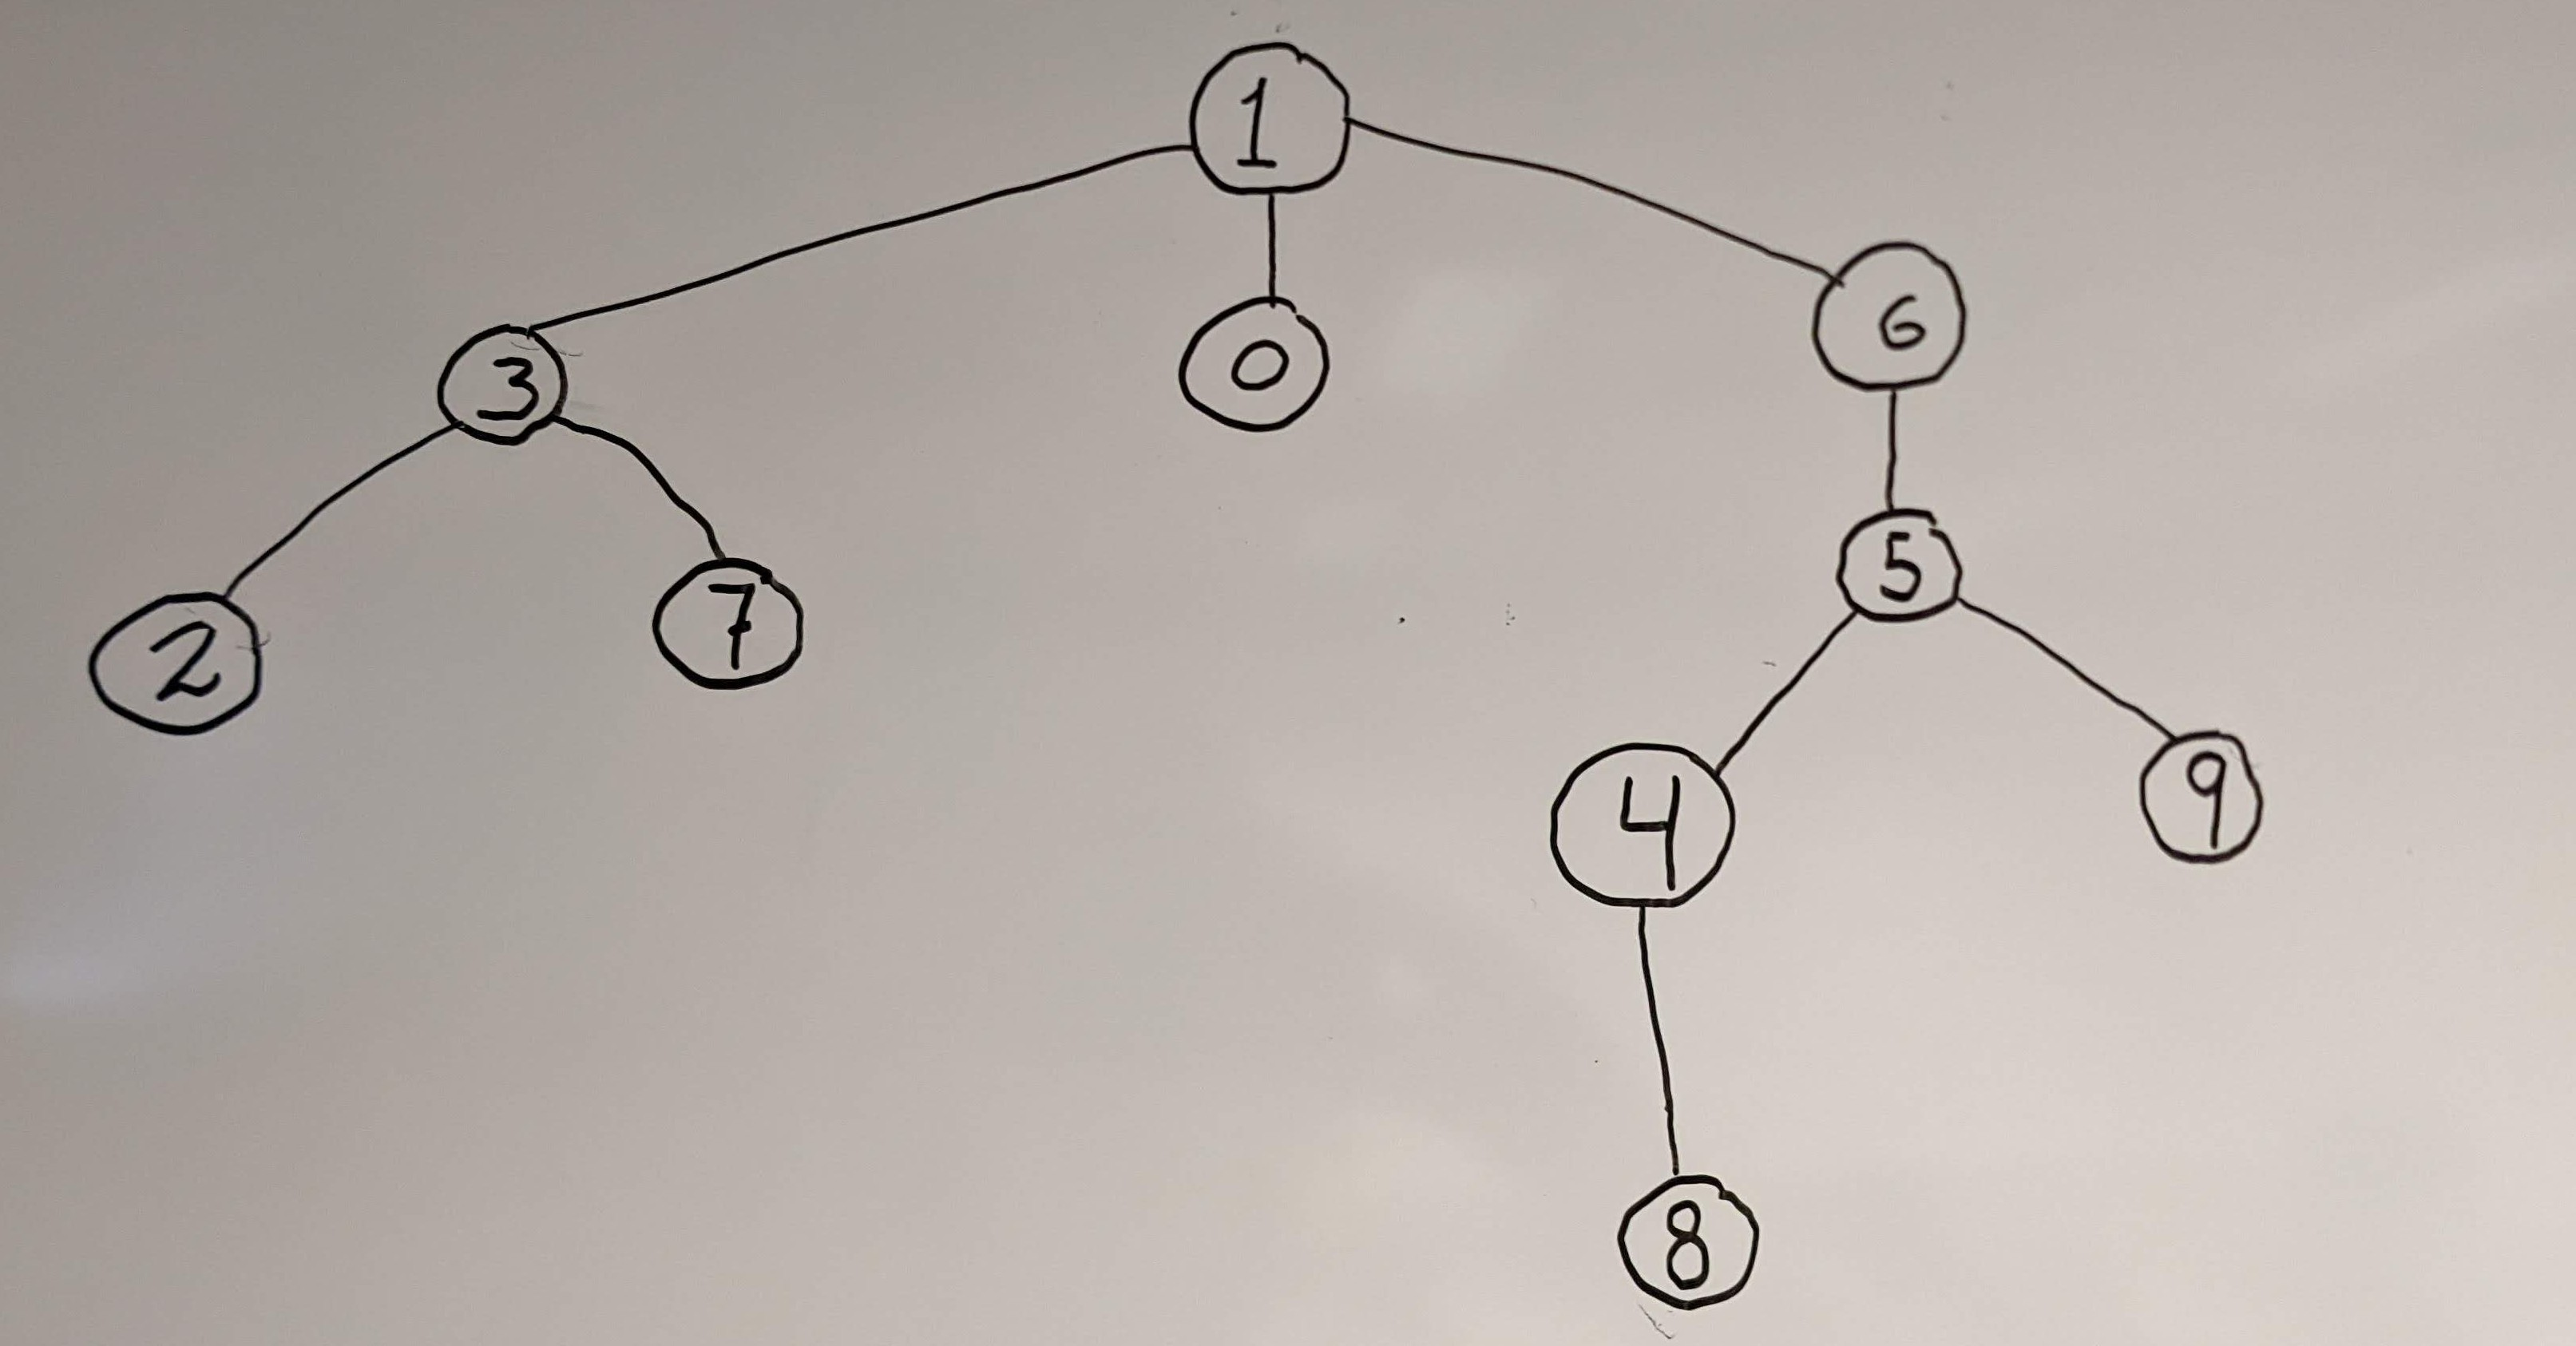
\includegraphics[scale=0.1]{imgs/tree_159.jpg}
\end{center}
þetta er ekki tré er ekki hægt að búa til með \emph{WQU} vegna þess, 
eins og sést á myndinni fyrir ofan, 
hefur $5$ sem er barn $6$ fleiri börn en $6$ og getur þessvegna ekki verið barn þess. 
\textbf{Réttari mynd væri með enga tengingu á milli 5 og 6.}

\section*{5.1.12}
\begin{lstlisting}
    public class WeightedQuickUnionUF {
    private int[] id; // parent link (site indexed)
    private int[] sz; // size of component for roots (site indexed)
    private int count; // number of components

    public WeightedQuickUnionUF(int N) {
        count = N;
        id = new int[N];
        for (int i = 0; i < N; i++)
            id[i] = i;
        sz = new int[N];
        for (int i = 0; i < N; i++)
            sz[i] = 1;
    }

    public int count() {
        return count;
    }

    /**
     * athugar hvort p se gild rot
     * 
     * @param p rot til ad athuga
     * @return skilar true ef rotin er gild
     */
    private boolean isRoot(int p) {
        int n = id.length;
        if (p >= n || p < 0)
            return false;
        return true;
    }

    public boolean connected(int p, int q) {
        return find(p) == find(q);
    }

    private int find(int p) { // Follow links to find a root.
        if (!isRoot(p))
            throw new IllegalArgumentException("Ekki gild rot");

        // geymir upprunalega p
        int root = p;
        while (p != id[p]) {
            p = id[p];
        }

        // tekur p og faerir thad upp i efstu rot
        while (root != p) {
            int temp = id[root];
            id[root] = p;
            root = temp;
        }
        return p;
    }

    public void union(int p, int q) {
        int i = find(p);
        int j = find(q);
        if (i == j)
            return;
        // Make smaller root point to larger one.
        if (sz[i] < sz[j]) {
            id[i] = j;
            sz[j] += sz[i];
        } else {
            id[j] = i;
            sz[i] += sz[j];
        }
        count--;
    }

    public static void main(String[] args) {
        int n = StdIn.readInt();
        WeightedQuickUnionUF uf = new WeightedQuickUnionUF(n);
        while (!StdIn.isEmpty()) {
            int p = StdIn.readInt();
            int q = StdIn.readInt();
            if (uf.find(p) == uf.find(q)) {
                continue;
            }
            uf.union(p, q);
            StdOut.println(p + " " + q);
        }
        StdOut.println(uf.count() + " components");
    }
}

\end{lstlisting}

\end{document}